%!TeX root=../solnQCQI.tex

\chapter{Quantum error-correction}

\Textbf{10.1} Verify that the encoding circuit in Figure 10.2 works as claimed:
\begin{center}
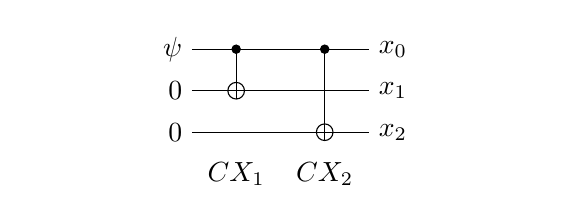
\begin{tikzpicture}[scale=1.000000,x=1pt,y=1pt]
\filldraw[color=white] (0.000000, -7.500000) rectangle (64.000000, 37.500000);
% Drawing wires
% Line 1: a1 W \ket{\psi} x_0
\draw[color=black] (0.000000,30.000000) -- (64.000000,30.000000);
\draw[color=black] (0.000000,30.000000) node[left] {$\ket{\psi}$};
% Line 2: a2 W \ket{0} x_1
\draw[color=black] (0.000000,15.000000) -- (64.000000,15.000000);
\draw[color=black] (0.000000,15.000000) node[left] {$\ket{0}$};
% Line 3: a3 W \ket{0} x_2
\draw[color=black] (0.000000,0.000000) -- (64.000000,0.000000);
\draw[color=black] (0.000000,0.000000) node[left] {$\ket{0}$};
% Done with wires; drawing gates
% Line 4: a1 +a2 width=20%% $CX_1$
\draw (16.000000, -7.500000) node[text width=144pt,below,text centered] {$CX_1$};
\draw (16.000000,30.000000) -- (16.000000,15.000000);
\filldraw (16.000000, 30.000000) circle(1.500000pt);
\begin{scope}
\draw[fill=white] (16.000000, 15.000000) circle(3.000000pt);
\clip (16.000000, 15.000000) circle(3.000000pt);
\draw (13.000000, 15.000000) -- (19.000000, 15.000000);
\draw (16.000000, 12.000000) -- (16.000000, 18.000000);
\end{scope}
% Line 5: a1 +a3 width=20%% $CS_2$
\draw (48.000000, -7.500000) node[text width=144pt,below,text centered] {$CX_2$};
\draw (48.000000,30.000000) -- (48.000000,0.000000);
\filldraw (48.000000, 30.000000) circle(1.500000pt);
\begin{scope}
\draw[fill=white] (48.000000, 0.000000) circle(3.000000pt);
\clip (48.000000, 0.000000) circle(3.000000pt);
\draw (45.000000, 0.000000) -- (51.000000, 0.000000);
\draw (48.000000, -3.000000) -- (48.000000, 3.000000);
\end{scope}
% Done with gates; drawing ending labels
\draw[color=black] (64.000000,30.000000) node[right] {$x_0$};
\draw[color=black] (64.000000,15.000000) node[right] {$x_1$};
\draw[color=black] (64.000000,0.000000) node[right] {$x_2$};
% Done with ending labels; drawing cut lines and comments
% Done with comments
\end{tikzpicture}
\end{center}
\Soln Let $\ket{\psi} = a\ket{0}+b\ket{1}$.  Our goal is to show that application of the diagrammed circuit maps $\ket{\psi}\ket{00} = a\ket{000}+b\ket{100}$ to $a\ket{000}+b\ket{111} = a\ket{0_L}+b\ket{1_L}$.  Note that $\ket{\psi}\ket{00} = \begin{bmatrix}a & 0 & 0 & 0 & b & 0 & 0 & 0\end{bmatrix}^T$, and $$CX_1 = \begin{bmatrix}1 & 0 & 0 & 0 & 0 & 0 & 0 & 0 \\ 0 & 1 & 0 & 0 & 0 & 0 & 0 & 0 \\ 0 & 0 & 1 & 0 & 0 & 0 & 0 & 0 \\ 0 & 0 & 0 & 1 & 0 & 0 & 0 & 0 \\ 0 & 0 & 0 & 0 & 0 & 0 & 1 & 0 \\ 0 & 0 & 0 & 0 & 0 & 0 & 0 & 1 \\ 0 & 0 & 0 & 0 & 1 & 0 & 0 & 0 \\ 0 & 0 & 0 & 0 & 0 & 1 & 0 & 0\end{bmatrix},\ 
CX_2 = \begin{bmatrix}1 & 0 & 0 & 0 & 0 & 0 & 0 & 0 \\ 0 & 1 & 0 & 0 & 0 & 0 & 0 & 0 \\ 0 & 0 & 1 & 0 & 0 & 0 & 0 & 0 \\ 0 & 0 & 0 & 1 & 0 & 0 & 0 & 0 \\ 0 & 0 & 0 & 0 & 0 & 1 & 0 & 0 \\ 0 & 0 & 0 & 0 & 1 & 0 & 0 & 0 \\ 0 & 0 & 0 & 0 & 0 & 0 & 0 & 1 \\ 0 & 0 & 0 & 0 & 0 & 0 & 1 & 0\end{bmatrix}.$$

So 
\begin{align*} CX_2CX_1\ket{\psi}\ket{00} &= \begin{bmatrix}1 & 0 & 0 & 0 & 0 & 0 & 0 & 0 \\ 0 & 1 & 0 & 0 & 0 & 0 & 0 & 0 \\ 0 & 0 & 1 & 0 & 0 & 0 & 0 & 0 \\ 0 & 0 & 0 & 1 & 0 & 0 & 0 & 0 \\ 0 & 0 & 0 & 0 & 0 & 1 & 0 & 0 \\ 0 & 0 & 0 & 0 & 1 & 0 & 0 & 0 \\ 0 & 0 & 0 & 0 & 0 & 0 & 0 & 1 \\ 0 & 0 & 0 & 0 & 0 & 0 & 1 & 0\end{bmatrix}\begin{bmatrix}1 & 0 & 0 & 0 & 0 & 0 & 0 & 0 \\ 0 & 1 & 0 & 0 & 0 & 0 & 0 & 0 \\ 0 & 0 & 1 & 0 & 0 & 0 & 0 & 0 \\ 0 & 0 & 0 & 1 & 0 & 0 & 0 & 0 \\ 0 & 0 & 0 & 0 & 0 & 0 & 1 & 0 \\ 0 & 0 & 0 & 0 & 0 & 0 & 0 & 1 \\ 0 & 0 & 0 & 0 & 1 & 0 & 0 & 0 \\ 0 & 0 & 0 & 0 & 0 & 1 & 0 & 0\end{bmatrix}\begin{bmatrix}a \\ 0 \\ 0 \\ 0 \\ b \\ 0 \\ 0 \\ 0\end{bmatrix} \\
&=\begin{bmatrix}a & 0 & 0 & 0 & 0 & 0 & 0 & b\end{bmatrix}^T \\ 
&= a\ket{000}+b\ket{111}
\end{align*}
as desired.